\subsection{\acs*{cadx}: Feature detection} \label{subsec:chp3:img-clas:CADX-fea-dec}

Discriminative features which help to recognize \ac{cap} from healthy tissue need to be first detected.
This processing is known in computer vision as feature extraction. 
However, feature extraction also refers to the name given in pattern recognition to some types of dimension reduction methods which are later presented.
In order to avoid confusion between these two aspects, in this survey, the procedure ``detecting'' or ``extracting'' features from images and signals is defined as feature detection.
This section summarizes the different features used in \ac{cad} for \ac{cap}.

\subsubsection{Image-based features}\label{subsubsec:chp3:img-clas:CADX-fea-dec:Img-fea}

This section focuses on image-based features which can be categorized into two categories: (i) voxel-wise detection and (ii) region-wise detection.

\paragraph{Voxel-wise detection}
This strategy refers to the fact that a feature is extracted at each voxel location.
As discussed in \acs{chp}\,\ref{chap:2}, \ac{cap} has an influence on the \ac{si} in \ac{mpmri} images.
Therefore, intensity-based feature is the most commonly used feature~\cite{Ampeliotis2007,Ampeliotis2008,Vos2008,rampun2016computerb,rampun2015classifying,Giannini2013,Artan2009,Artan2010,Chan2003,Langer2009,Litjens2011,Litjens2012,Litjens2014,Liu2009,Ozer2009,Ozer2010,trigui2016classification,trigui2017automatic,cameron2014multiparametric,cameron2016maps,khalvati2015automated,chung2015prostate,giannini2015fully,Niaf2011,Niaf2012,lehaire2014computer}.
This feature consists in the extraction of the intensity of the \ac{mri} modality of interest.

Edge-based features have also been used to detect \ac{si} changes but bring additional information regarding the \ac{si} transition.
Each feature is computed by convolving the original image with an edge operator.
Three operators are commonly used: (i) Prewitt operator~\cite{Prewitt1970}, (ii) Sobel operator~\cite{Sobel1970}, and (iii) Kirsch operator~\cite{Kirsch1971}.
These operators differ due to the kernel used which attenuates more or less the noise.
Multiple studies used the resulting magnitude and orientation of the edges computed in their classification frameworks~\cite{Niaf2011,Niaf2012,Tiwari2009a,Tiwari2010,Tiwari2013,Viswanath2008,Viswanath2011,rampun2016quantitative,rampun2015computer,rampun2016computer,lehaire2014computer,khalvati2015automated,chung2015prostate}.

\begin{figure}
	\hspace*{\fill}
		\subfigure[$\theta=0^{\circ}$.]{\label{subfig:gab1} 
\includegraphics[width=0.2\linewidth]{3_review/figures/feature-detection/gabor/gabor_1.eps}} \hfill
		\subfigure[$\theta=60^{\circ}$.]{\label{subfig:gab2} 
\includegraphics[width=0.2\linewidth]{3_review/figures/feature-detection/gabor/gabor_2.eps}} \hfill
		\subfigure[$\theta=120^{\circ}$.]{\label{subfig:gab3} 
\includegraphics[width=0.2\linewidth]{3_review/figures/feature-detection/gabor/gabor_3.eps}} \hfill
		\subfigure[$\theta=180^{\circ}$.]{\label{subfig:gab4} 
\includegraphics[width=0.2\linewidth]{3_review/figures/feature-detection/gabor/gabor_4.eps}}
	\hspace*{\fill}
	\caption[Illustration of 4 different Gabor filters.]{Illustration of 4 different Gabor filters varying their orientations $\theta$.}
	\label{fig:gabor}
\end{figure}

Gabor filters~\cite{Gabor1946,Daugman1985} offer an alternative to the usual edge detector, with the possibility to tune the direction and the frequency of the filter to encode a specific pattern. 
A Gabor filter is defined by the modulation of a Gaussian function with a sine wave which can be further rotated and is formalized as in \acs{eq}\,\ref{eq:gabor}.
\begin{equation}
	g(x,y;\theta,\psi,\sigma,\gamma) = \exp \left( - \frac{x'^{2}+ \gamma^{2}y'^{2}}{2 \sigma^{2}} \right) \cos \left( 2 \pi \frac{x'}{\lambda} + \psi \right) \ ,
        \label{eq:gabor}
\end{equation}

\noindent with 

\begin{eqnarray}
	x' & = & s\left( x \cos \theta + y \sin \theta \right) \ , \nonumber \\
	y' & = & s \left( - x \sin \theta + y \cos \theta \right) \ , \nonumber
\end{eqnarray}

\noindent where $\lambda$ is the wavelength of the sinusoidal factor, $\theta$ represents the orientation of the Gabor filter, $\psi$ is the phase offset, $\sigma$ is the standard deviation of the Gaussian envelope, $\gamma$ is the spatial aspect ratio, and $s$ is the scale factor.
In an effort to characterize pattern and texture, a bank of Gabor filters is usually created with different angles, scale, and frequency --- refer to \acs{fig}\,\ref{fig:gabor} --- and then convolved with the image.
\citeauthor{Viswanath2012}~\cite{Viswanath2012}, \citeauthor{Tiwari2012}~\cite{Tiwari2012} and more recently \citeauthor{khalvati2015automated}~\cite{khalvati2015automated} and \citeauthor{chung2015prostate}~\cite{chung2015prostate} have designed a bank of Gabor filters to characterized texture and edge information in \ac{t2w}-\ac{mri} and \ac{dw}-\ac{mri} modalities.

Texture-based features provide other characteristics discerning \ac{cap} from healthy tissue.
The most common texture analysis for image classification is based on the \ac{glcm} with their related statistics which have been proposed by \citeauthor{Haralick1973} in~\cite{Haralick1973}.
In a neighborhood around a central voxel, a \ac{glcm} is build considering each voxel pair defined by a specific distance and angle.
Then, using the \ac{glcm}, a set of statistical features is computed as defined in \acs{tab}~\ref{tab:glcm} and assigned to the location of the central voxel.
Therefore, $N$ --- up to 14 --- statistical maps are derived from the \ac{glcm} analysis, one per statistics presented in \acs{tab}~\ref{tab:glcm}.
\ac{glcm} is commonly used in \ac{cad} systems, on the different \ac{mri} modalities, namely \ac{t2w}-\ac{mri}, \ac{dce}-\ac{mri}, or \ac{dw}-\ac{mri}~\cite{Antic2013,Niaf2011,Niaf2012,Tiwari2009a,Tiwari2010,Tiwari2013,Viswanath2008,Viswanath2009,Viswanath2011,Viswanath2012,trigui2016classification,rampun2015computer,rampun2016computer,rampun2016quantitative,cameron2014multiparametric,cameron2016maps,khalvati2015automated,chung2015prostate,lehaire2014computer}.
However, the statistics extracted from the \ac{glcm} across studies vary.
Along the same line, \citeauthor{rampun2016computer} extracted from \ac{t2w}-\ac{mri}~\cite{rampun2016computer,rampun2015computer} Tamura features~\cite{tamura1978textural} composed of three features to characterize texture: (i) coarseness, (ii) contrast, and (iii) directionality.

\begin{table}
  \caption[The 14 statistical features used in conjunction with \acs*{glcm} analysis.]{The 14 statistical features for texture analysis commonly computed from the \acs*{glcm} $p$ as presented by~\cite{Haralick1973}.}
  \scriptsize
  \renewcommand{\arraystretch}{1.5}
  \centering
  \begin{tabular}{ll}
    \toprule
    \textbf{Statistical features} & \textbf{Formula} \\
    \midrule
    Angular second moment & $\sum_i \sum_j p(i,j)^2 $  \\
    Contrast & $\sum_{n=0}^{N_g - 1} n^2 \left[ \sum_{i=1}^{N_g - 1} \sum_{j=1}^{N_g - 1} p(i,j) \right] \ , | i-j |=n  $ \\
    Correlation & $\frac{\sum_i \sum_j (ij) p(i,j) - \mu_x \mu_y}{\sigma_x \sigma_y}  $ \\
    Variance & $\sum_i \sum_j (i - \mu)^2 p(i,j)  $ \\
    Inverse difference moment & $\sum_i \sum_j \frac{1}{1+(i - \mu)^2} p(i,j)  $ \\
    Sum average & $\sum_{i=2}^{2N_g} i p_{x+y}(i)  $ \\
    Sum variance & $\sum_{i=2}^{2N_g} (i-f_s)^2 p_{x+y}(i)  $ \\
    Sum entropy & $ - \sum_{i=2}^{2N_g} p_{x+y}(i) \log p_{x+y}(i)  $ \\
    Entropy & $ - \sum_i \sum_j p(i,j) \log p(i,j) $ \\
    Difference variance & $\sum_{i=0}^{N_g-1} i^2 p_{x-y}(i)  $ \\
    Difference entropy & $ - \sum_{i=0}^{N_g-1} p_{x-y}(i) \log p_{x-y}(i)  $ \\
    Info. measure of corr. 1 & $\frac{S(X;Y)-S_1(X;Y)}{\max(S(X),S(Y))}  $ \\
    Info. measure of corr. 2 & $\sqrt{\left( 1 - \exp \left[ -2( H_2(X;Y) - H(X;Y) ) \right] \right)}  $ \\
    Max. corr. coeff. & $ \sqrt{\lambda_2} \ , \text{of } Q(i,j) = \sum_k \frac{p(i,k)p(j,k)}{p_x(i)p_y(k)}  $ \\
    \bottomrule
  \end{tabular}
  \label{tab:glcm}
\end{table}

\citeauthor{Lopes2011} used fractal analysis  and more precisely a local estimation of the fractal dimension~\cite{Benassi1998}, to describe the texture roughness at a specific location.
The fractal dimension is estimated through a wavelet-based method in multi-resolution analysis.
They showed that cancerous tissues have a higher fractal dimension than healthy tissue.

\citeauthor{Chan2003} described texture using the frequency signature via the \acf{dct}\cite{Ahmed1974} defining a neighbourhood of \SI[product-units=repeat]{7x7}{\px} for modalities used, namely \ac{t2w}-\ac{mri} and \ac{dw}-\ac{mri}.
The \ac{dct} allows to decompose a portion of an image into a coefficient space, where few of these coefficients encode the significant information.
The \ac{dct} coefficients are computed such as:

\begin{equation}
	C_{k_1,k_2} = \sum_{m=0}^{M-1} \sum_{n=0}^{N-1} p_{m,n} \cos \left[ \frac{\pi}{M} \left( m + \frac{1}{2} \right) k_1 \right] \cos \left[ \frac{\pi}{N} \left( n + \frac{1}{2} \right) k_2 \right] \ ,
\end{equation}

\noindent where $C_{k_1,k_2}$ is the \ac{dct} coefficient at the position $k_1,k_2$, $M$ and $N$ are the dimension of the neighbourhood and $p_{m,n}$ is the pixel \ac{si} at the position $\{m,n\}$.

Regarding other features, \citeauthor{Viswanath2012} projected \ac{t2w}-\ac{mri} images into the wavelet space, using the Haar wavelet, and used the resulting coefficients as features~\cite{Viswanath2012}.
%The wavelet family used for the decomposition was the Haar wavelet.
\citeauthor{Litjens2011} computed the texture map based on \ac{t2w}-\ac{mri} images using a Gaussian filter bank~\cite{Litjens2011}.
Likewise, \citeauthor{rampun2016computer} employed a rotation invariant filter bank proposed in~\cite{leung2001representing}.
The bank is composed of 48 filters including Gaussian filters, first and second derivatives of Gaussian filters as well as Laplacian of Gaussian.

%% Euclidean distance from each voxel to the prostate center as well as the individual distance in the three directions $x$, $y$ and $z$. \cite{Chan2003} embedded the same information but this time using cylindrical coordinate $r$, $\theta$ and $z$ corresponding to the radius, azimuth and elevation respectively.

\paragraph{Region-wise detection}

Unlike the previous section, another strategy is to study a region instead of each pixel independently.
Usually, the feature maps are computed using the method presented in voxel-based approach followed by a step in which features are computed in some specific delineated regions to characterize them.

The most common feature type is based on statistics and more specifically the statistic-moments such as mean, standard deviation, kurtosis, and skewness~\cite{Ampeliotis2007,Ampeliotis2008,Tiwari2009a,Tiwari2010,Tiwari2013,Viswanath2008,Viswanath2009,Viswanath2012,rampun2016quantitative,rampun2015computer,rampun2016computer,Antic2013,Viswanath2011,Peng2013,cameron2014multiparametric,cameron2016maps,khalvati2015automated,chung2015prostate,Litjens2011,Litjens2012,Litjens2014,Niaf2011,Niaf2012,lehaire2014computer}.
Additionally, some studies extract additional statistical landmarks based on percentiles~\cite{Vos2008a,Antic2013,Peng2013,Vos2010,Litjens2011,Litjens2012,Litjens2014,Niaf2011,Niaf2012,Vos2012,lehaire2014computer}
The percentiles to use are manually determined by observing the \ac{pdf} of the features and checking which values allow the best to differentiate malignant from healthy tissue.

Further statistics are computed through the use of histogram-based features.
\citeauthor{Liu2013} introduced 4 different types of histogram-based features to characterize hand-delineated lesions~\cite{Liu2013}.
The first type corresponds to the histogram of the \ac{si} of the image.
The second type is the \ac{hog}~\cite{Dalal2005} which encodes the local shape of the object of interest by using the distribution of the gradient directions.
This descriptor is extracted mainly in three steps.
First, the gradient image and its corresponding magnitude and direction are computed.
Then, the \ac{roi} is divided into cells and an oriented-based histogram is generated for each cell.
At each pixel location, the orientation of the gradient votes for a bin of the histogram and this vote is weighted by the magnitude of the same gradient.
Finally, the cells are grouped into blocks and each block is normalized.
The third histogram-based type used in~\cite{Liu2013} is the shape context introduced in~\cite{Belongie2002}.
The shape context is also a way to describe the shape of an object of interest.
First, a set of points defining edges have to be detected and for each point of each edge, a log-polar-based histogram is computed using the relative points distribution.
The last set of histogram-based feature extracted is based on the framework described in~\cite{Zhao2012} which is using the Fourier transform of the histogram created via \acf{lbp}~\cite{Ojala1996}.
\Ac{lbp} is generated by comparing the value of the central pixel with its neighbours, defined through a radius and the number of connected neighbours.
Then, in the \ac{roi}, the histogram of the \ac{lbp} distribution is computed.
The \acf{dft} of the \ac{lbp} histogram is used to make the feature invariant to rotation.

Another subset of features are anatomical-based features and have been used in~\cite{Litjens2012,Litjens2014,Matulewicz2013,cameron2014multiparametric,cameron2016maps}.
\citeauthor{Litjens2012} computed the volume, compactness, and sphericity related to the given region~\cite{Litjens2012, Litjens2014}.
Additionally, \citeauthor{Litjens2014} also introduced a feature based on symmetry in which they compute the mean of a candidate lesion as well as its mirrored counter-part and compute the quotient as feature~\cite{Litjens2014}.
\citeauthor{Matulewicz2013} introduced 4 features corresponding to the percentage of tissue belonging to the regions \ac{pz}, \ac{cg}, periurethral region, or outside the prostate region for the considered \ac{roi}~\cite{Matulewicz2013}.
Finally, \citeauthor{cameron2016maps} defined 4 features based on morphology and asymmetry:
(i) the difference of morphological closing and opening of the \ac{roi}, (ii) the difference of the initial perimeter and the one after removing the high-frequency components, (iii) the difference between the initial \ac{roi} and the one after removing the high-frequency components, and (iv) the asymmetry by computing the difference of the two areas splitting the \ac{roi} by its major axes~\cite{cameron2014multiparametric,cameron2016maps}.

The last group of region-based feature is based on fractal analysis.
This group of features is based on estimating the fractal dimension which is a statistical index representing the complexity of the analyzed texture.
\citeauthor{Lv2009} proposed two features based on fractal dimension: (i) texture fractal dimension and (ii) histogram fractal dimension~\cite{Lv2009}.
The first feature is based on estimating the fractal dimension on the \ac{si} of each image and thus this feature is a statistical characteristic of the image roughness.
The second fractal dimension is estimated using the \ac{pdf} of each image and characterizes the complexity of the \ac{pdf}.
\citeauthor{Lopes2011} proposed a 3D version to estimate the fractal dimension of a volume using a wavelet decomposition~\cite{Lopes2011}.

\subsubsection{\acs*{dce}-based features}\label{subsubsec:chp3:img-clas:CADX-fea-dec:DCE-fea}

\ac{dce}-\ac{mri} is more commonly based on a \ac{si} analysis over time as presented in \acs{sec}\,\ref{subsec:chp2:imaging:dce}.
In this section, the specific features extracted for \ac{dce}-\ac{mri} analysis are presented.

\begin{table}
  \caption{Parameters used as features for a \acs*{dce} semi-quantitative analysis in \acs*{cad} systems.}
  \scriptsize
  \centering
  \begin{tabularx}{\textwidth}{l X}
    \toprule
    \textbf{Semi-quantitative features} & \textbf{Explanations} \\
    \midrule
    \textbf{Amplitude features:} & \\ \\ [-1.5ex]
    \quad $S_0$ & Amplitude at the onset of the enhancement \\
    \quad $S_{\max}$ & Amplitude corresponding to $95\%$ of the maximum amplitude \\
    \quad $S_{p}$ & Amplitude corresponding to the maximum amplitude \\
    \quad $S_f$ & Amplitude at the final time point \\ \\ [-1.5ex]
    \textbf{Time features:} & \\ \\ [-1.5ex]
    \quad $t_0$ & Time at the onset of the enhancement \\
    \quad $t_{\max}$ & Time corresponding to $95\%$ of the maximum amplitude \\
    \quad $t_{p}$ & Time corresponding to the maximum amplitude \\
    \quad $t_{f}$ & Final time \\
    \quad $t_{tp}$ & Time to peak which is the time from $t_0$ to $t_p$ \\ \\ [-1.5ex]
    \textbf{Derivatives and integral features:} & \\ \\ [-1.5ex]
    \quad $WI$ & Wash-in rate corresponding to the signal slope from $t_0$ to $t_m$ or $t_p$ \\
    \quad $WO$ & Wash-out rate corresponding to the signal slope from $t_m$ or $t_p$ to $t_p$ \\
    \quad $IAUC$ & Initial area under the curve which is the area between $t_0$ to $t_{f}$ \\
    \bottomrule
  \end{tabularx}
\label{tab:semiqua}
\end{table}

\paragraph{Whole-spectra approach}
Some studies are using the whole \ac{dce} time series as feature vector~\cite{Ampeliotis2007,Ampeliotis2008,Tiwari2012,Viswanath2008a,Viswanath2008}.
In some cases, the high-dimensional feature space is reduced using dimension reduction methods as it will be presented in the \acs{sec}\,\ref{subsec:chp3:img-clas:CADX-fea-ext}.

\begin{figure}
  \centering
  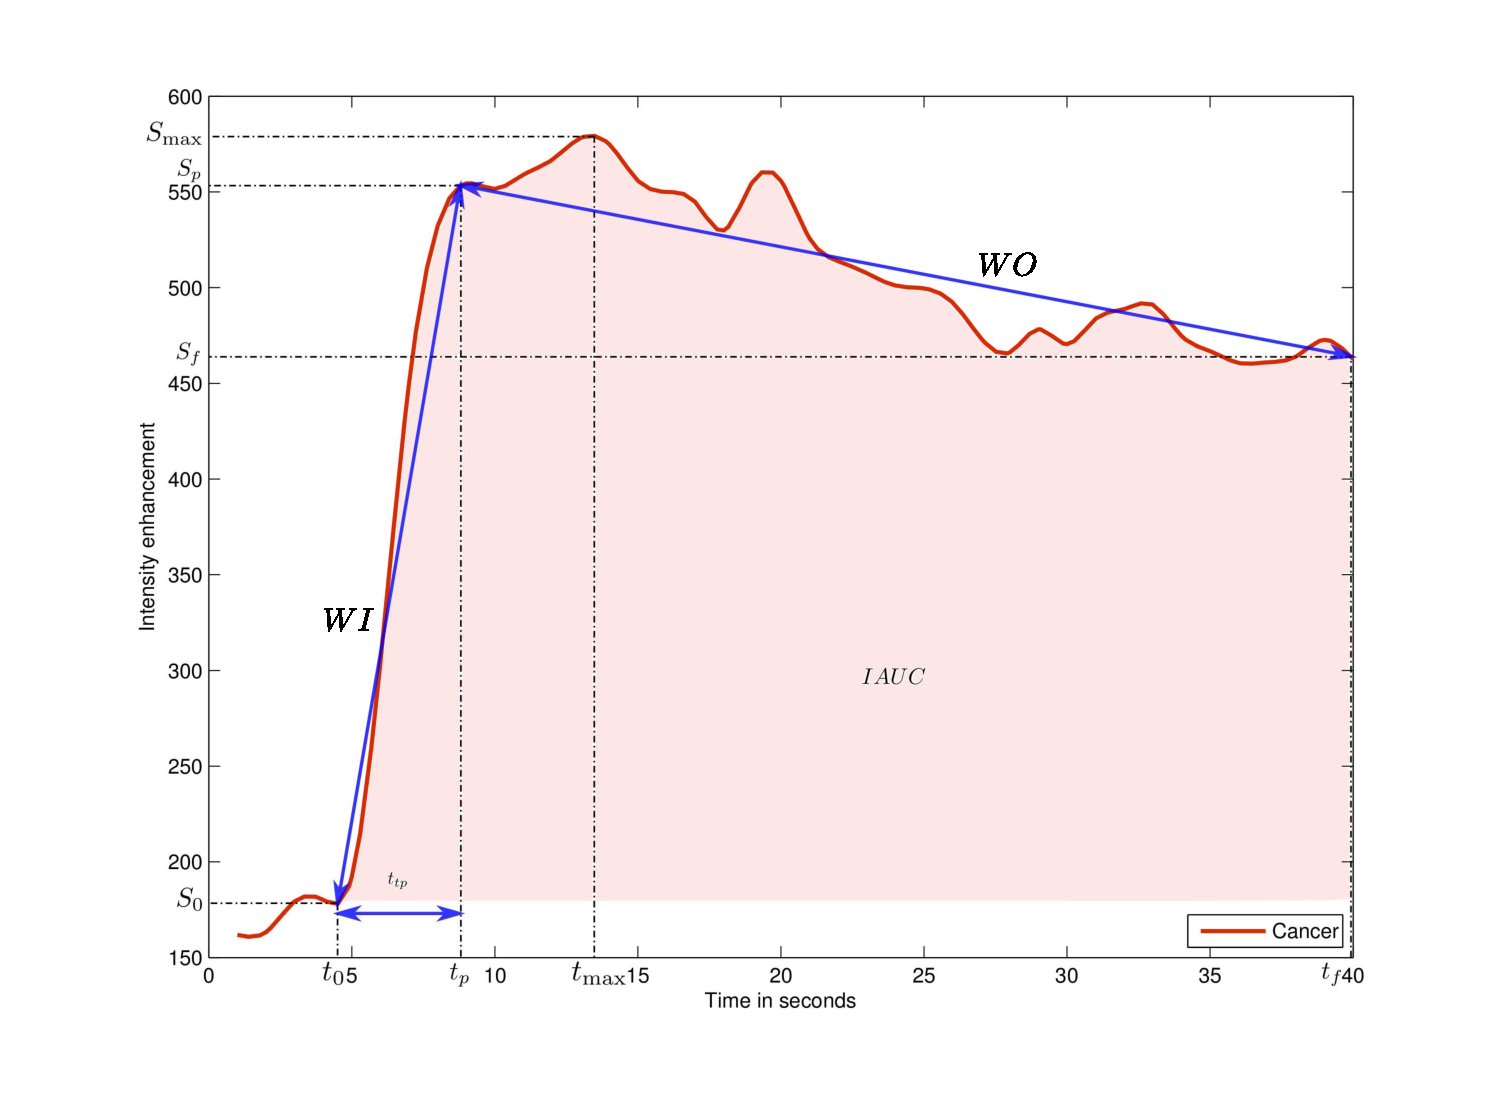
\includegraphics[width=.8\linewidth]{3_review/figures/feature-detection/dce/dce_cancer_parameters.eps}
  \caption[Semi-quantitative features used for \acs*{dce}-\acs*{mri}.]{Graphical representation of the different semi-quantitative features used for \acs*{dce}-\acs*{mri} analysis.}
  \label{fig:dceparam}
\end{figure}

\paragraph{Semi-quantitative approach}
Semi-quantitative approaches are based on mathematically modelling the \ac{dce} time series.
The parameters modelling the signal are commonly used, mainly due to the simplicity of their computation~\cite{Puech2009,Mazzetti2011,Niaf2011,Niaf2012,Sung2011,trigui2016classification,trigui2017automatic,lehaire2014computer,samarasinghe2016semi,giannini2015fully}.
Parameters included in semi-quantitative analysis are summarized in \acs{tab}~\ref{tab:semiqua} and also graphically depicted in \acs{fig}\,\ref{fig:dceparam}.
A set of time features corresponding to specific amplitude level (start, maximum, and end) are extracted.
Then, derivative and integral features are also considered as discriminative and are commonly computed.

\paragraph{Quantitative approach}
As presented in \acs{chp}\,\ref{chap:2}, quantitative approaches correspond to mathematical-pharmacokinetic models based on physiological exchanges.
Four different models have been used in \ac{cad} for \ac{cap} systems.
The most common model reviewed is the \textit{Brix model}~\cite{Artan2009,Artan2010,Sung2011,Liu2009,Ozer2009,Ozer2010}.
This model is formalized such as:
\begin{equation}
	\frac{S(t)}{S(0)} = 1 + A k_{ep} \left( \frac{\exp( -k_{ep} t ) - \exp( -k_{el} t )}{k_{el} - k_{ep}} \right) \ ,
	\label{eq:brixmod}
\end{equation}

\noindent where $S(\cdot)$ is the \ac{dce} signal, $A$ is the parameter simulating the tissue properties, $k_{el}$ is the parameter related to the first-order elimination from the plasma compartment, and $k_{ep}$ is the parameter of the transvascular permeability.
The parameters $k_{ep}$, $k_{el}$, and $A$ are computed from the \ac{mri} data and used as features.

Another model is Tofts model~\cite{Tofts1997} which has been used in~\cite{Langer2009,Giannini2013,Niaf2011,Niaf2012,Mazzetti2011,lehaire2014computer,giannini2015fully}.
In this model, the \ac{dce} signal relative to the concentration is presented as:
\begin{equation}
	C_t(t) = v_p C_p(t) + K_{trans} \int_{0}^{t} C_p(\tau) \exp( -k_{ep}(t-\tau) ) \ d\tau \ ,
	\label{eq:tofts} 
\end{equation}

\noindent where $C_t(\cdot)$ is the concentration of the medium, $C_p(\cdot)$ is the \ac{aif} which has to be estimated independently, $K_{trans}$ is the parameter related to the diffuse transport of media across the capillary endothelium, $k_{ep}$ is the parameter related to the exchanges back into the vascular space, and $v_e$ is the extravascular-extracellular space fraction defined such that $v_e = 1 - v_p$.
In this model, parameters $K_{trans}$, $k_{ep}$, and $v_e$ are computed and used as features.

\citeauthor{Mazzetti2011} and \citeauthor{giannini2015fully} used the Weibull function~\cite{Mazzetti2011,Giannini2013,giannini2015fully} which is formalized as:

\begin{equation}
	S(t) = A t \exp( -t^{B} ) \ ,
	\label{eq:weibull}
\end{equation}

\noindent where $A$ and $B$ are the two parameters which have to be inferred.

They also used another empirical model which is based on the West-like function and named the \ac{pun}~\cite{Castorina2006}, formalized as:
\begin{equation}
	S(t) = \exp \left[ r t + \frac{1}{\beta} a_0 - r \left( \exp( \beta t ) - 1 \right) \right] \ ,
	\label{eq:pun}
\end{equation}
\noindent where the parameters $\beta$, $a_0$ and $r$ are inferred.
For all these models, the parameters are inferred using an optimization curve fitting approach.

\subsubsection{\acs*{mrsi}-based features}\label{subsubsec:chp3:img-clas:CADX-fea-dec:MRSI-fea}

\paragraph{Whole spectra approach}
As in the case of \ac{dce} analysis, one common approach is to incorporate the whole \ac{mrsi} spectra in the feature vector for classification~\cite{Kelm2007,Parfait2012,Tiwari2007,Tiwari2009,Tiwari2013,Tiwari2009a,Tiwari2010,Viswanath2008a,Matulewicz2013,trigui2016classification,trigui2017automatic}.
Sometimes post-processing involving dimension reduction methods is performed to reduce the complexity during the classification as it will be presented in \acs{sec}\,\ref{subsec:chp3:img-clas:CADX-fea-ext}.

\paragraph{Quantification approach}
We can reiterate that in \ac{mrsi} only few biological markers --- i.e., choline, creatine, and citrate metabolites --- are known to be useful to discriminate \ac{cap} and healthy tissue.
Therefore, only the concentrations of these metabolites are considered as a feature prior to classification.
In order to perform this quantification, 4 different approaches have been used.
\citeauthor{Kelm2007} used the following models~\cite{Kelm2007}: QUEST~\cite{Ratiney2005}, AMARES~\cite{Vanhamme1997}, and VARPRO~\cite{Coleman1993}.
They are all time-domain quantification methods varying by the type of pre-knowledge embedded and the optimization approaches used to solve the quantification problem.
Unlike the time-domain quantification approaches, \citeauthor{Parfait2012} used the LcModel approach proposed in~\cite{Provencher1993} which solves the optimization problem in the frequency domain.
Although \citeauthor{Parfait2012} used each metabolite relative concentration individually~\cite{Parfait2012}, other authors such as \citeauthor{Kelm2007} proposed to compute relative concentrations as the ratios of metabolites as shown in \acs{eq}\,\ref{eq:ratio1} and \acs{eq}\,\ref{eq:ratio2}.

\begin{eqnarray}
	R_1 & = & \frac{ [ \text{Cho} ] + [ \text{Cr} ]}{[ \text{Cit} ]} \ . \label{eq:ratio1} \\
	R_2 & = & \frac{[ \text{Cit} ]}{[\text{Cho}]+[\text{Cr}]+[\text{Cit}]} \ , \label{eq:ratio2}
\end{eqnarray}
\noindent where $\text{Cit}$, $\text{Cho}$ and $\text{Cr}$ are the relative concentration of citrate, choline, and creatine, respectively.

Recently \citeauthor{trigui2017automatic} used an absolute quantification approach from which water sequences are acquired to compute the absolute concentration of the metabolites~\cite{trigui2016classification,trigui2017automatic}.
Absolute quantification using water as reference is based on the fact that the fully relaxed signal from water or metabolites is proportional to the number of moles of the molecules in the voxel~\cite{gasparovic2006use}.

\paragraph{Wavelet decomposition approach} 
\citeauthor{Tiwari2012} performed a wavelet packet decomposition~\cite{Coifman1992} of the spectra using the Haar wavelet basis function and use its coefficients as features.

\subsubsection{Summary}

The feature detection methods used in \ac{cad} are summarized in \acs{tab}~\ref{tab:feat}.  

%%%% THIS TABLE NEEDS TO BE CHANG
\newgeometry{margin=1cm}
\thispagestyle{empty}
\begin{table}
  \centering
  \caption{Overview of the feature detection methods used in \ac{cad} systems.}\label{tab:feat}
  \footnotesize
  \begin{threeparttable}
    \renewcommand{\arraystretch}{.7}
    \begin{tabular}{p{.5\linewidth} p{.4\linewidth}}
      \hline \\ [-1.5ex]
      \textbf{Feature detection methods} & \textbf{Indexes} \\ \\ [-1.5ex]
      \hline \\ [-1.5ex]
      \textbf{\ac{mri} image:} & \\ \\ [-1.5ex]
      \quad \textit{Voxel-wise detection} &  \\ \\ [-1.5ex]
      \quad \quad Intensity-based & $^{\text{{\cmarksmall}- -}}$\cite{Ampeliotis2007,Ampeliotis2008,Vos2008}\par $^{\text{- - {\cmarksmall}}}$\cite{Giannini2013}\par $^{\text{{\cmarksmall}- {\cmarksmall}}}$\cite{Artan2009,Artan2010,Chan2003,Langer2009,Litjens2011,Litjens2012,Litjens2014,Liu2009,Ozer2009,Ozer2010}\par $^{\text{{\cmarksmall}{\cmarksmall}{\cmarksmall}}}$\cite{Niaf2011,Niaf2012} \\ 
      \quad \quad Edge-based & \\
      \quad \quad \quad Prewitt operator & $^{\text{{\cmarksmall}- -}}$\cite{Tiwari2009a,Tiwari2010,Tiwari2013,Viswanath2008} \\
      \quad \quad \quad Sobel operator & $^{\text{{\cmarksmall}- -}}$\cite{Tiwari2009a,Tiwari2010,Tiwari2013,Viswanath2008,Viswanath2009,Viswanath2011,Viswanath2012}\par $^{\text{{\cmarksmall}{\cmarksmall}{\cmarksmall}}}$\cite{Niaf2011,Niaf2012} \\
      \quad \quad \quad Kirsch operator & $^{\text{{\cmarksmall}- -}}$\cite{Tiwari2009a,Tiwari2010,Tiwari2013,Viswanath2008,Viswanath2009,Viswanath2011,Viswanath2012}\par $^{\text{{\cmarksmall}{\cmarksmall}{\cmarksmall}}}$\cite{Niaf2011,Niaf2012} \\
      \quad \quad \quad Gabor filtering & $^{\text{{\cmarksmall}- -}}$\cite{Tiwari2012,Viswanath2008,Viswanath2012} \\ 
      \quad \quad Texture-based & \\
      \quad \quad \quad Haralick features & $^{\text{{\cmarksmall}- -}}$\cite{Antic2013,Tiwari2009a,Tiwari2010,Tiwari2013,Viswanath2008,Viswanath2009,Viswanath2012}\par $^{\text{{\cmarksmall}{\cmarksmall}-}}$\cite{Viswanath2011}\par $^{\text{{\cmarksmall}{\cmarksmall}{\cmarksmall}}}$\cite{Litjens2012,Niaf2011,Niaf2012} \\
      \quad \quad \quad Fractal analysis & $^{\text{{\cmarksmall}- -}}$\cite{Lopes2011,Lv2009} \\
      \quad \quad \quad \Ac{dct} & $^{\text{{\cmarksmall}{\cmarksmall}{\cmarksmall}}}$\cite{Chan2003} \\
      \quad \quad \quad Wavelet-based features & $^{\text{{\cmarksmall}- -}}$\cite{Viswanath2012} \\
      \quad \quad \quad Gaussian filter bank & $^{\text{{\cmarksmall}- -}}$\cite{Litjens2014} \\ 
      \quad \quad Position-based & \cite{Chan2003,Litjens2011,Litjens2012,Litjens2014} \\ \\ [-1.5ex]
      \quad \textit{Region-wise detection} &  \\ \\ [-1.5ex]
      \quad \quad Statistical-based & \\
      \quad \quad \quad Percentiles & $^{\text{- {\cmarksmall}-}}$\cite{Vos2008a} \par $^{\text{- - {\cmarksmall}}}$\cite{Antic2013,Peng2013}\par $^{\text{{\cmarksmall}{\cmarksmall}-}}$\cite{Vos2010}\par $^{\text{{\cmarksmall}{\cmarksmall}{\cmarksmall}}}$\cite{Litjens2011,Litjens2012,Litjens2014,Niaf2011,Niaf2012,Vos2012} \\
      \quad \quad \quad Statistical-moments & $^{\text{{\cmarksmall}- -}}$\cite{Ampeliotis2007,Ampeliotis2008,Tiwari2009a,Tiwari2010,Tiwari2013,Viswanath2008,Viswanath2009,Viswanath2012}\par $^{\text{- - {\cmarksmall}}}$\cite{Antic2013}\par $^{\text{{\cmarksmall}{\cmarksmall}-}}$\cite{Viswanath2011}\par $^{\text{{\cmarksmall}- {\cmarksmall}}}$\cite{Peng2013}\par $^{\text{{\cmarksmall}{\cmarksmall}{\cmarksmall}}}$\cite{Litjens2011,Litjens2012,Litjens2014,Niaf2011,Niaf2012} \\
      \quad \quad Histogram-based & \\
      \quad \quad \quad \acs{pdf} & $^{\text{{\cmarksmall}{\cmarksmall}{\cmarksmall}}}$\cite{Liu2013} \\
      \quad \quad \quad \acs{hog} & $^{\text{{\cmarksmall}{\cmarksmall}{\cmarksmall}}}$\cite{Liu2013} \\
      \quad \quad \quad Shape context & $^{\text{{\cmarksmall}{\cmarksmall}{\cmarksmall}}}$\cite{Liu2013} \\
      \quad \quad \quad \acs{lbp} & $^{\text{{\cmarksmall}{\cmarksmall}{\cmarksmall}}}$\cite{Liu2013} \\
      \quad \quad Anatomical-based & \cite{Litjens2012,Litjens2014,Matulewicz2013} \\ \\ [-1.5ex]
      \textbf{\ac{dce} signal:} & \\ \\ [-1.5ex]
      \quad Whole spectra approach & \cite{Ampeliotis2007,Ampeliotis2008} \\
      \quad Semi-quantitative approach & $^{\text{{\mmarksmall}}}$\cite{Puech2009}\par \cite{Mazzetti2011,Niaf2011,Niaf2012,Sung2011} \\
      \quad Quantitative approach &  \\
      \quad \quad Toft model & $^{\text{{\mmarksmall}}}$\cite{Liu2013,Peng2009}\par \cite{Giannini2013,Langer2009,Litjens2011,Litjens2012,Litjens2014,Mazzetti2011,Niaf2011,Niaf2012} \\
      \quad \quad Brix model & $^{\text{{\mmarksmall}}}$\cite{Artan2009,Artan2010,Ozer2009,Ozer2010}\par \cite{Liu2009,Sung2011} \\
      \quad \quad Weibull function & \cite{Giannini2013,Mazzetti2011} \\
      \quad \quad PUM & \cite{Giannini2013,Mazzetti2011} \\
      \\ [-1.5ex]
      \textbf{\ac{mrsi} signal:} & \\ \\ [-1.5ex]
      \quad Whole spectra approach & \cite{Kelm2007,Matulewicz2013,Parfait2012,Tiwari2007,Tiwari2008,Tiwari2009,Tiwari2009a,Tiwari2010,Tiwari2013,Viswanath2008} \\
      \quad Quantification approach & \cite{Kelm2007,Parfait2012} \\
      \quad Wavelet-based approach & \cite{Tiwari2012} \\ \\ [-1.5ex]
      \hline
    \end{tabular}
    \begin{tablenotes}
      \footnotesize
    \item Notes:
    \item ( {\cmarksmall}$|$- {\cmarksmall}$|$- {\cmarksmall}$|$- ): triplet stating the implementation or not of the feature for respectively \ac{t2w}-\ac{mri} images, \ac{dce}-\ac{mri} images, \ac{dw}-\ac{mri} images.
    \item {\cmarksmall}: used or implemented.
    \item {\mmarksmall}: partially implemented.
    \end{tablenotes}
  \end{threeparttable}
\end{table}
\restoregeometry


